\documentclass[10pt]{standalone}
\usepackage{amsmath}
\usepackage{amssymb}
\usepackage{pgf,tikz}
\usepackage{mathrsfs}
\usetikzlibrary{arrows,calc,positioning,shapes.symbols,shapes.geometric,shapes.misc}
\pagestyle{empty}
\usepackage{siunitx}

\begin{document}
	
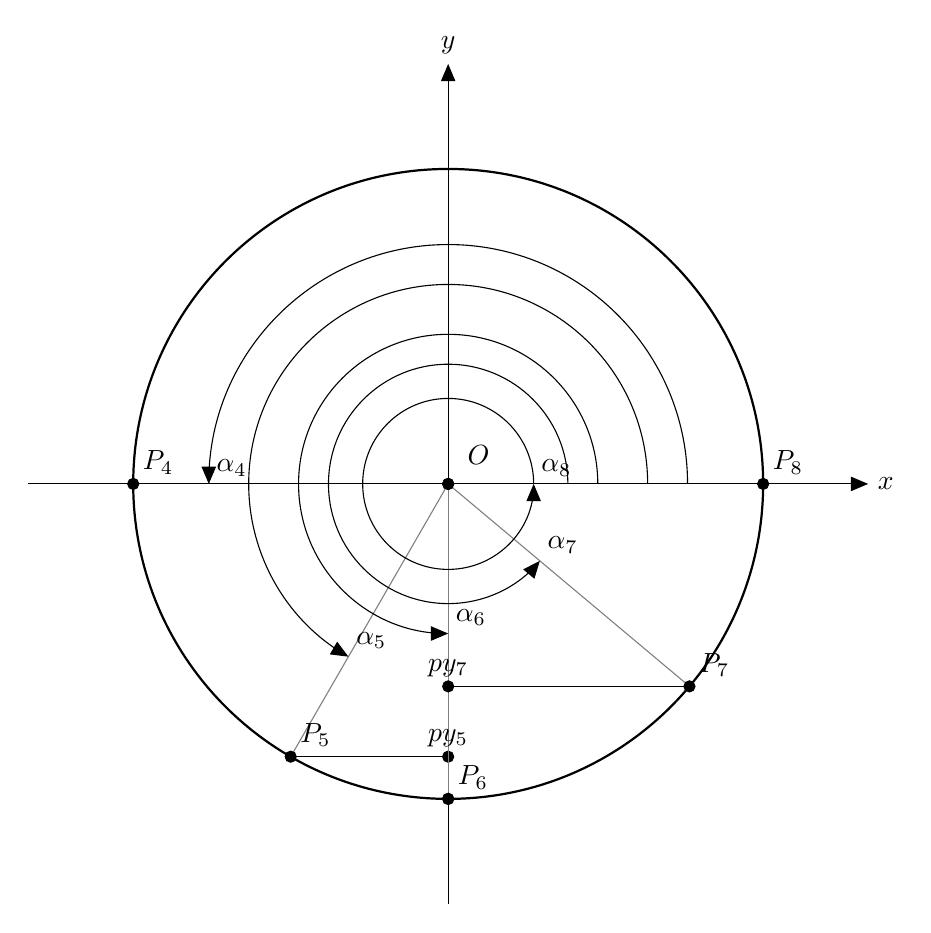
\begin{tikzpicture}[>=triangle  45] %, x=0.8cm,y=0.8cm]
% draw the coordinates
\pgfmathsetmacro{\raggio}{4};
\pgfmathsetmacro{\mraggio}{\raggio/3};
\pgfmathsetmacro{\qraggio}{\raggio/5};
\pgfmathsetmacro{\sraggio}{1.9*\raggio};
% draw the unit circle
\draw[->] (0,-\raggio-\mraggio) -- (0,\raggio+\mraggio) node[above,fill=white] {$y$};
\draw[->] (-\raggio-\mraggio,0) -- (\raggio+\mraggio,0) node[right,fill=white] {$x$};
\draw[thick] (0,0) circle(\raggio);
%\draw (-\raggio-\qraggio-0.2,0) node[above=1pt] {$(-1,0)$}
%(\raggio+\qraggio,0)  node[above=1pt] {$(1,0)$}
%(0,-\raggio-\qraggio-0.2) node[fill=white] {$(0,-1)$}
%(0,\raggio+\qraggio+0.2)  node[fill=white] {$(0,1)$};
\node(OO)at(0,0) [label= above right:$O$] {};
\foreach \x in {180,240,270,320,360}{
	% lines from center to point
	\draw[gray] (0,0) -- (\x:\raggio);
	% dots at each point
	\filldraw[black] (\x:\raggio) circle(2pt);
	% draw each angle in degrees
	%\draw (\x:0.8*\raggio) node[fill=white] {$\x^\circ$};
	\draw(\x:\raggio)--($((0,-1)!(\x:\raggio)!(0,1)$);
	\filldraw[black] ($((0,-1)!(\x:\raggio)!(0,1)$) circle(2pt);
}
\foreach \x/ \y/\arco  in {
	180/2.5/{\alpha_4},
	240/3/{\alpha_5},
	270/4/{\alpha_6},
	320/5/{\alpha_7},
	%150/6,
	360/7 /{\alpha_8}%,
	%210/8,
	%240/9,
	%270/10,
	%300/11,
	%330/12,
	%360/13
}
\draw[->] (\sraggio/\y,0 ) arc (0:\x:\sraggio/\y) node[above right=-1pt] {$\arco$};
\foreach \x/ \y in {
	%180/ py_4,	
	%30/px_1,	
	240/py_5,
	%270/py_6,
	320/py_7
	%,
	%150/px_5,
	%360/py_8	 %,
	%210/8,
	%240/9,
	%270/10,
	%300/11,
	%330/12,
	%360/13
}
\draw ($((0,-1)!(\x:\raggio)!(0,1)$) node[above] {$\y$};
\foreach \x/ \y in {
	180/ P_4,	
	%30/P_1,	
	240/P_5,
	270/P_6,
	320/P_7,
	%150/P_8,
	360/P_8 %,
	%210/8,
	%240/9,
	%270/10,
	%300/11,
	%330/12,
	%360/13
}
\draw ( \x:\raggio) node[above  right] {$\y$};
\end{tikzpicture}
\end{document}